\hyperdef{}{tilda}{}

\subsection{Operatoren}


\par\noindent\textbf{\href{http://de.wikipedia.org/wiki/Operator_(Mathematik)}{Wikipedia
zu Operatoren in der Mathematik}}

\begin{quote}
Ein Operator ist eine mathematische Vorschrift (ein Kalkül), durch die
man aus mathematischen Objekten neue Objekte bilden kann. Er kann eine
standardisierte Funktion oder eine Vorschrift über Funktionen sein.
Anwendung finden die Operatoren bei Rechenoperationen, also bei
manuellen oder bei maschinellen Berechnungen.
\end{quote}



\par\noindent\textbf{\href{http://de.wikipedia.org/wiki/Operator_(Logik)}{Wikipedia
zu Operatoren in der Logik}}

\begin{quote}
Ein Logischer Operator ist eine Funktion, die einen Wahrheitswert
liefert. Bei der zweiwertigen, booleschen Logik liefert er also wahr
oder falsch, bei einer mehrwertigen Logik können auch entsprechend
andere Werte geliefert werden.
\end{quote}


\subsubsection{Allgemeines}

\par\noindent\textbf{Vereinfachte Begriffserklärung}

\begin{itemize}
\itemsep1pt\parskip0pt\parsep0pt
\item
  {Wenn wir uns den Operator als einen Verfertiger von Objekten
  vorstellen, dann heißt das, dass ein Operator \emph{irgendetwas} mit
  \emph{irgendetwas} anstellt. Entscheidend sind hierbei die Fragen,
  \emph{was} der Operator tut, und \emph{womit} der Operator etwas tut.}
\item
  {Ein Operator wandelt also eines oder mehrere Objekte in neue Objekte
  um.}
\item
  {Das, was umgewandelt wird, nennen wir die \emph{Operanden} eines
  Operators.}
\item
  {Das, was der Operator mit den Operanden tut, nennen wir die
  \emph{Operation}.}
\item
  {Der Plus-Operator wandelt bspw. zwei Zahlen in eine Zahl um, indem er
  die Operation \emph{Addition} ausführt.}
\end{itemize}



\par\noindent\textbf{Klassifikation von Operatoren}

{Operatoren können nach verschiedenen Kriterien klassifiziert werden.
Die grundlegendste Unterscheidung besteht in der Anzahl der Operanden,
auf die ein Operator die Operation anwendet. Hierbei unterscheiden wir
zwischen \emph{unären} und \emph{binären} Operatoren}

\begin{itemize}
\itemsep1pt\parskip0pt\parsep0pt
\item
  {\emph{Unäre} Operatoren haben nur einen Operanden.}
\item
  {\emph{Binäre} Operatoren haben zwei Operanden.}
\end{itemize}



\par\noindent\textbf{Klassifikation von Operatoren}

{Ferner kann zwischen \emph{arithmetischen}, \emph{logischen} und
\emph{relationalen} Operatoren unterschieden werden.}

\begin{itemize}
\itemsep1pt\parskip0pt\parsep0pt
\item
  {\emph{Arithmentische} Operatoren führen arithmetische Operationen aus
  (Addition, Division, etc.).}
\item
  {\emph{Logische} Operatoren liefern Aussagen über Wahrheitswerte (wahr
  oder falsch).}
\item
  {\emph{Relationale} Operatoren liefern Aussagen über die Beziehungen
  zwischen Objekten (Identität, Zugehörigkeit).}
\end{itemize}



\par\noindent\textbf{Überladen von Operatoren}

\begin{itemize}
\itemsep1pt\parskip0pt\parsep0pt
\item
  {Normalerweise werden Operatoren immer nur für spezifische Datentypen
  definiert.}
\item
  {Der Operator \$+\$ nimmt als Operanden bspw. gewöhnlich nur Zahlen.}
\item
  {In vielen Programmiersprachen ist es jedoch üblich, Operatoren, je
  nach Datentyp, auf den sie angewendet werden, unterschiedliche
  Operationen zuzuschreiben.}
\item
  {Diesen Vorgang nennt man das \emph{Überladen} von Operatoren.}
\item
  {Wird der Additionsoperator \$+\$ bswp. auf den Datentyp \emph{string}
  angewendet, so bewirkt er eine Verkettung von Strings
  (Konkatenation).}
\item
  {Das Überladen von Operatoren ermöglicht es, sehr kompakt und flexibel
  zu programmieren.}
\end{itemize}


\subsubsection{\ldots{} in Python}

\par\noindent\textbf{Allgemeines}

\begin{itemize}
\itemsep1pt\parskip0pt\parsep0pt
\item
  {Die Operatoren in Python ähneln denen vieler Programmiersprachen.}
\item
  {Neben den durch mathematische Zeichen dargestellten Operatoren
  (\$+\$, \$-\$, \$*\$) sind einige Operatoren auch als \emph{Namen}
  (\textbf{is}, \textbf{in}) definiert.}
\item
  {Die Überladung von Operatoren ist ein entscheidender Wesenszug der
  Sprache. Viele Operatoren sind auf viele Datentypen anwendbar.}
\end{itemize}




\par\noindent\textbf{Arithmetische Operatoren}

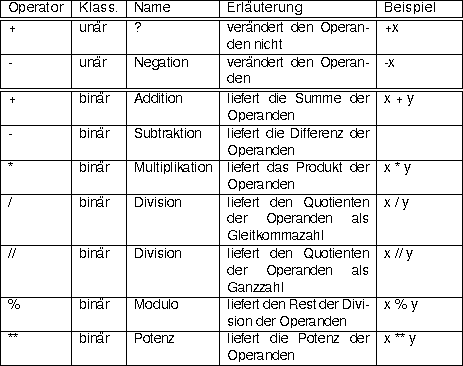
\includegraphics[width=\textwidth]{img/operatoren.pdf}




\par\noindent\textbf{Arithmetische Operatoren}

\begin{verbatim}
>>> x,y = 5,2
>>> +x
5
>>> -x
-5
>>> x + y
7
>>> x - y
3
>>> x * y
10
>>> x / y
2.5
>>> x // y
2
>>> x % y
1
>>> x ** y
25
\end{verbatim}




\par\noindent\textbf{Logische Operatoren}

\begin{itemize}
\itemsep1pt\parskip0pt\parsep0pt
\item
  {Die logischen Operatoren dienen dem Verarbeiten von Wahrheitswerten.}
\item
  {Jeder Wert bekommt in Python automatisch einen Wahrheitswert
  zugewiesen (\textbf{True} oder \textbf{False}).}
\item
  {Die Wahrheitswerte werden dem Datentyp \emph{bool} zugeschrieben.}
\item
  {Negative Zahlen einschließlich der Zahl \$0\$ besitzen den
  Wahrheitswert \textbf{False}.}
\item
  {Alle ``leeren'' Werte (der leere String \texttt{""} oder die leere
  Liste \texttt{{[}{]}}) besitzen ebenfalls den Wahrheitswert
  \textbf{False}.}
\item
  {Die logischen Operatoren prüfen den Wahrheitswert von Werten und
  liefern als Ergebnis einen Wahrheitswert zurück.}
\end{itemize}




\par\noindent\textbf{Logische Operatoren}

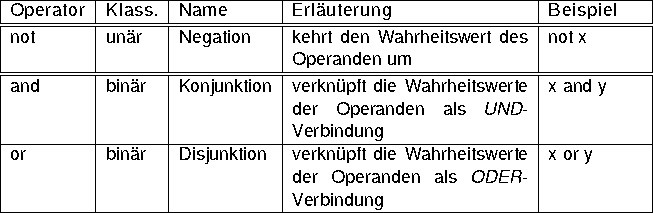
\includegraphics[width=\textwidth]{img/logische_operatoren.pdf}




\par\noindent\textbf{Logische Operatoren}

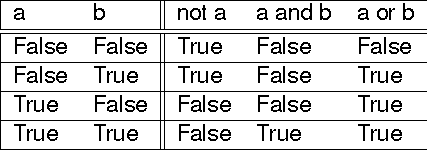
\includegraphics[width=\textwidth]{img/truth_table.pdf}




\par\noindent\textbf{Logische Operatoren}

Wenn andere Werte als der Datentyp \emph{bool} mit den Operatoren
\par\noindent\textbf{and} und \textbf{or} verknüpft werden, so wird immer einer der
beiden Operanden zurückgegeben, wobei die Bedingungen für die Rückgabe
wie folgt sind:

\begin{itemize}
\itemsep1pt\parskip0pt\parsep0pt
\item
  {{[}\textbf{and}{]}}

  \begin{itemize}
  \itemsep1pt\parskip0pt\parsep0pt
  \item
    {Wenn der erste Operand falsch ist, wird dieser zurückgegeben.}
  \item
    {Wenn der erste Operand wahr ist, wird der zweite Operand
    zurückgegeben.}
  \end{itemize}
\item
  {{[}\textbf{or}{]}}

  \begin{itemize}
  \itemsep1pt\parskip0pt\parsep0pt
  \item
    {Wenn der erste Operand wahr ist, wird dieser zurückgegeben.}
  \item
    {Wenn der erste Operand falsch ist, wird der zweite Operand
    zurückgegeben.}
  \end{itemize}
\end{itemize}




\par\noindent\textbf{Logische Operatoren}

\begin{verbatim}
>>> x,y = True,False
>>> not x
False
>>> not y
True
>>> x and y
False
>>> x or y
True
>>> x,y = False,False
>>> not x and not y
True
>>> x and y
False
>>> x or y
False
>>> x,y = 'harry','potter'
>>> x and y
'potter'
>>> x or y
'harry'
>>> x = False
>>> x and y
False
>>> x or y
'potter'
\end{verbatim}




\par\noindent\textbf{Relationale Operatoren}

\begin{itemize}
\itemsep1pt\parskip0pt\parsep0pt
\item
  {Relationale Operatoren liefern immer einen Wahrheitswert in Bezug auf
  die Relation zurück, die überprüft werden soll.}
\item
  {Bei den relationalen Operatoren kann zwischen Vergleichs-, Element-
  und Identitätsoperatoren unterschieden werden.}

  \begin{itemize}
  \itemsep1pt\parskip0pt\parsep0pt
  \item
    {Vergleichsoperatoren dienen dem Vergleich von Operanden
    hinsichtlich ihrer Werte.}
  \item
    {Zugehörigkeitsoperatoren dienen der Ermittlung der Zugehörigkeit
    eines Operanden zu anderen Operanden.}
  \item
    {Identitätsoperatoren dienen der Ermittlung von
    Identitätsverhältnissen, wobei Identität von Gleichheit ähnlich
    abgegrenzt wird wie dies im Deutschen mit Hilfe der Wörter
    \emph{dasselbe} vs. \emph{das gleiche} getan wird.}
  \end{itemize}
\end{itemize}




\par\noindent\textbf{Relationale Operatoren}

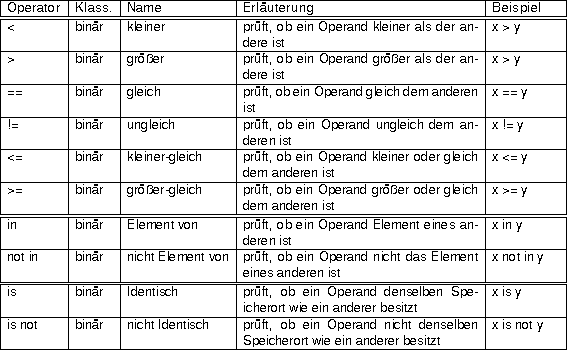
\includegraphics[width=\textwidth]{img/relationale_operatoren.pdf}




\par\noindent\textbf{Relationale Operatoren: Vergleichsoperatoren}

\begin{verbatim}
>>> x,y = 5,10
>>> x > y
False
>>> x < y
True
>>> x == y
False
>>> x != y
True
>>> x <= y
True
>>> x >= y
False
\end{verbatim}




\par\noindent\textbf{Relationale Operatoren: Zugehörigkeitsoperatoren}

\begin{verbatim}
>>> x,y = 'doculect','cul'
>>> x in y
False
>>> y in x
True
>>> x not in y
True
\end{verbatim}




\par\noindent\textbf{Relationale Operatoren: Identitätsoperatoren}

\begin{verbatim}
>>> x = 1,2
>>> y = x
>>> x is y
True
>>> y = 1,2
>>> x is y
False
\end{verbatim}




\par\noindent\textbf{Arithmetische Operatoren}

Die arithmetischen Operatoren in JavaScript sind im Großen und Ganzen
identisch mit denen in Python. Lediglich der Potenz-Operator \texttt{**}
existiert nicht.




\par\noindent\textbf{Arithmetische Operatoren}

\begin{verbatim}
> var x = 5; var y = 2;
> +x;
5
> -x;
-5
> x + y;
7
> x - y;
3
> x * y;
10
> x / y;
2.5
> x // y;
2
> x % y;
1
> Math.pow(x,y); // x ** y in Python
25
\end{verbatim}




\par\noindent\textbf{Logische Operatoren}

Funktionell sind die logischen Operatoren in JavaScript identisch mit
denen in Python, jedoch werden an Stelle der Schlüsselwörter
\par\noindent\textbf{and}, \textbf{or} und \textbf{not} in JavaScript die Zeichen
\par\noindent\textbf{\textbackslash{}\&\textbackslash{}\&},
\par\noindent\textbf{\textbar{}\textbar{}} und \textbf{!} verwendet. Ferner werden
die beiden Werte des Datentyps \textbf{bool} klein geschrieben
(\textbf{true} und \textbf{false} anstelle von \textbf{True} und
\par\noindent\textbf{False}).




\par\noindent\textbf{Logische Operatoren}

\begin{verbatim}
> var x = true; var y = false
> !x; // not x in Python
false
> !y // not y in Python
true
> x && y // x and y in Python
false
> x || y // x or y in Python
true
> var x = false; var y = false;
> ! x && ! y // not x and not y in Python
true
> x && y
false
> x || y
false
> var x = 'harry'; var y = 'potter';
> x && y
'potter'
> x || y
'harry'
> var x = False
> var x && y
false
>>> x || y
'potter'
\end{verbatim}




\par\noindent\textbf{Relationale Operatoren}

Auch die relationalen Operatoren in JavaScript sind denen in Python sehr
ähnlich. Es fehlen jedoch die Operatoren \textbf{in} und \textbf{not
in}. Anstelle der Schlüsselwörter \textbf{is} und \textbf{is not} werden
die Symbole \textbf{===} und \textbf{!==} verwendet.




\par\noindent\textbf{Relationale Operatoren: Vergleichsoperatoren}

\begin{verbatim}
> var x = 5; var y = 10;
> x > y
false
> x < y
true
> x == y
false
> x != y
true
> x <= y
true
> x >= y
false
\end{verbatim}




\par\noindent\textbf{Relationale Operatoren: Vergleichsoperatoren}

\begin{verbatim}
> var x = 'doculect'; var y = 'cul';
> y.indexOf(x) != -1 // x in y in Python
false
> x.indexOf(y) != -1 // y in x in Python
true
> y.indexOf(x) == -1 // x not in y in Python
true
\end{verbatim}




\par\noindent\textbf{Relationale Operatoren: Vergleichsoperatoren}

\begin{verbatim}
> var x = [1, 2] // x = [1,2] in Python
> var y = x
> x === y // x is y in Python
true
> y = [1, 2] 
> x === y // x is y in Python
false
\end{verbatim}

\subsection{Kontrollstrukturen}

\subsubsection{Allgemeines}
\par\noindent\textbf{\href{http://de.wikipedia.org/wiki/Kontrollstruktur}{Gängige
Begriffserklärung aus Wikipedia}}

\begin{quote}
Kontrollstrukturen (Steuerkonstrukte) werden in imperativen
Programmiersprachen verwendet, um den Ablauf eines Computerprogramms zu
steuern. Eine Kontrollstruktur gehört entweder zur Gruppe der
Verzweigungen oder der Schleifen. Meist wird ihre Ausführung über
logische Ausdrücke der booleschen Algebra beeinflusst.
\end{quote}



\par\noindent\textbf{Begriffserklärung in
\href{http://bibliography.lingpy.org?key=Weigend2008}{Weigend
(2008:127)}}

\begin{quote}
Kontrollstrukturen legen fest, in welcher Reihenfolge und unter welchen
Bedingungen die Anweisungen eines Programms abgearbeitet werden.
\end{quote}



\par\noindent\textbf{Typen von Kontrollstrukturen}

\begin{itemize}
\itemsep1pt\parskip0pt\parsep0pt
\item
  {\textbf{Verzweigungen} kontrollieren den Fluss eines Programms, indem
  sie dieses, abhängig von bestimmten Gegebenheiten, in unterschiedliche
  Bahnen lenken}
\item
  {\textbf{Schleifen} kontrollieren den Fluss eines Programms, indem sie
  Operationen wiederholt auf Objekte anwenden}
\end{itemize}



\par\noindent\textbf{Typen von Kontrollstrukturen}

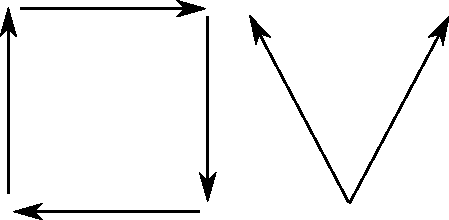
\includegraphics[width=\textwidth]{img/kontrollstrukturen.pdf}


\subsubsection{\ldots in Python}

\par\noindent\textbf{Allgemeines}

\begin{itemize}
\itemsep1pt\parskip0pt\parsep0pt
\item
  {Python kennt insgesamt vier verschiedene Kontrollstrukturen: zwei
  Verzweigungsstrukturen (\textbf{if}, \textbf{try}) und zwei
  Schleifenstrukturen (\textbf{for}, \textbf{while}).}
\item
  {Das besondere an den Kontrollstrukturen in Python ist deren enge
  Anbindung an logische Ausdrücke, welche einen sehr kompakten, sehr
  leicht verständlichen Kode erlauben.}
\end{itemize}


\par\noindent\textbf{Verzweigungen: if, elif, und else}

\begin{itemize}
\itemsep1pt\parskip0pt\parsep0pt
\item
  {Bei der \textbf{if}-Verzweigung wird ein Programmabschnitt unter
  einer bestimmten Bedingung ausgeführt.}
\item
  {Dabei wird eine Bedingung auf ihren Wahrheitswert getestet. Trifft
  sie zu, wird das Programm entsprechend weitergeführt. Trifft sie nicht
  zu, unterbleibt der Abschnitt.}
\item
  {Es können auch mehrere Bedingungen auf ihren Wahrheitswert überprüft
  und entsprechend mehrere verschiedene Programmabschnitte aktiviert
  werden.}
\item
  {Es gibt in Python auch die Möglichkeit, \emph{nichts} zu tun, wenn
  eine Bedingung zutrifft. Dies muss durch das Schlüsselwort
  \textbf{pass} festgelegt werden.}
\end{itemize}



\par\noindent\textbf{Verzweigungen: if, elif, und else}

\begin{verbatim}
>>> x, y, yes, no = 10, 0, "yes", "no"
>>> if x: print(yes)
yes
>>> if y: print(yes)
>>> if not x: print(yes)
    elif not y: print no
no
>>> if 1 > 10: print("Eins ist groesser als zehn.")
    elif 1 < 10: print("Eins ist kleiner als zehn.")
Eins ist kleiner als zehn.
>>> if x or y: print("Einer von beiden Werten ist wahr.")
    else: print("Keiner von beiden Werten ist wahr.")
Einer von beiden Werten ist wahr.
>>> if x == 10: pass
    else: print("Danke, Herr Jauch!")
\end{verbatim}


\par\noindent\textbf{Verzweigungen: try und except}

\begin{itemize}
\itemsep1pt\parskip0pt\parsep0pt
\item
  {Eine sehr wichtige und nützliche Verzweigunsstruktur bietet Python
  mit \textbf{try} und \textbf{except}.}
\item
  {Hierbei wird nicht eine Bedingung auf ihren Wahrheitswert überprüft,
  sondern getestet, ob ein Statement eine Fehlermeldung hervorruft.}
\item
  {Auf diese Weise kann man gezielt auf mögliche Fehler reagieren.}
\item
  {Fehler können dabei gezielt entsprechend ihrer Klasse eingeordnet
  werden.}
\item
  {Auf diese Weise können gezielt bestimmte Fehler angesprochen werden,
  die vom Programm ignoriert werden sollen.}
\end{itemize}



\par\noindent\textbf{Verzweigungen: try und except}

\begin{verbatim}
>>> try: x = int(input())
    except: print("Der Wert, den Sie eingegeben haben, ist kein Integer!")
2
>>> try: x = int(input())
    except ValueError: print("Der Wert, den Sie eingegeben haben, ist kein Integer!")
2.0
Der Wert, den Sie eingegeben haben, ist kein Integer!"
>>> x = input()
10
>>> x, y = 10, 0 
>>> try: x / y
    except ZeroDivisionError: print("Durch Null kann man nicht teilen!")
Durch Null kann man nicht teilen.
>>> try: x = int(input())
    except ValueError: print("Falscher Wert für Integer!")
10.0
Falscher Wert für Integer!
\end{verbatim}


\par\noindent\textbf{Schleifen: while}

\begin{itemize}
\itemsep1pt\parskip0pt\parsep0pt
\item
  {Mit Hilfe von Schleifenkonstruktionen werden Blöcke von Anweisungen
  in Programmen wiederholt ausgeführt, bis eine Abbruchsbedingung
  eintritt, bzw. so lange eine Bedingung zutrifft.}
\item
  {Wie für Verzweigunsstrukturen werden auch die Bedingungen in
  Schleifen auf Grundlage der Auswertung von Wahrheitswerten errechnet.}
\item
  {Der Abbruch einer Schleife kann in Python bewusst durch das
  Schlüsselwort \textbf{break} gesteuert werden.}
\end{itemize}




\par\noindent\textbf{Schleifen: while}

\begin{verbatim}
>>> a = 10
>>> while a > 0: 
        print(a," ist groesser als 0.")
        a -= 1 # wir lassen der Wert gegen 0 laufen

10 ist groesser als 0
9 ist groesser als 0
8 ist groesser als 0
7 ist groesser als 0
6 ist groesser als 0
5 ist groesser als 0
4 ist groesser als 0
3 ist groesser als 0
2 ist groesser als 0
1 ist groesser als 0
>>> while True:
        b = input("Sag was: ")
        print b
        if not b:
            print("Aaaaaabbbbbrrrrruuuuccccccch!")
            break
Sag was: bla
bla
Sag was: bloed
bloed
Aaaaaabbbbbrrrrruuuuccccccch!
\end{verbatim}




\par\noindent\textbf{Schleifen: for}

\begin{itemize}
\itemsep1pt\parskip0pt\parsep0pt
\item
  {Während bei der \textbf{while}-Schleife die Abbruchsbedingung immer
  explizit genannt werden muss, gilt dies nicht für die
  \textbf{for}-Schleife.}
\item
  {Hier wird explizit und im Voraus festgelegt, wie oft, bzw. in Bezug
  auf welche Objekte eine bestimmte Operation ausgeführt werden soll,
  weshalb sich die \textbf{for}-Schleife anbietet, wenn man die Anzahl
  der Operationen kennt, die man durchführen will.}
\item
  {Der Bereich, in dem in Python eine Operation mit Hilfe der
  \textbf{for}-Schleife ausgeführt wird, wird zumeist mit Hilfe der
  Funktion \textbf{range()} angegeben, welche automatisch eine Liste von
  Integern erzeugt, über die dann iteriert wird.}
\end{itemize}




\par\noindent\textbf{Schleifen: for}

\begin{verbatim}
>>> a = range(5)
>>> a
range(0,5)
>>> list(a)
[0, 1, 2, 3, 4]
>>> for i in range(5): print(i)
0
1
2
3
4
>>> einkaufsliste = ['mehl','butter','zitronen','bier']
>>> for element in einkaufsliste: print element
mehl
butter
zitronen
bier
>>> namen = ['peter','frank','karl','jan']
>>> for name in namen: print(name)
peter
frank
karl
jan
>>> woerter = ['haus','kaffee','getraenk','wasser','flasche']
>>> for wort in woerter: print(wort)
haus
kaffee
getraenk
wasser
flasche
\end{verbatim}


\subsubsection{\ldots{} in JavaScript}

\par\noindent\textbf{Verzweigungen: if, else if und else}

Die if-else-Verzweigung in JavaScript unterscheidet sich in ihrer Syntax
von Python, nicht jedoch in der grundlegenden Konzeption, auf der sie
aufbaut. Auch in JavaScript wird der Wahrheitswert einer Datenstruktur
getestet und entsprechend reagiert. Anstelle von ``elif'' wird dabei in
javaScript ``else if'' geschrieben. Ferner werden hässliche Klammern
verwendet anstelle der schönen Einrückungen, die in Python verwendet
werden.




\par\noindent\textbf{Verzweigungen: if, else if und else}

\begin{verbatim}
> var x = 10; var y = 0; var yes = 'yes'; var no = 'no';
> if (x) {console.log(yes);} // if x: print(yes) in Python
yes
> if (y) {console.log(yes);} // if y: print(yes) in Python 
>>> if (!x) {console.log(yes);}
    else if(!y) { console.log(no);}
no
>>> if (1 > 10) {console.log("Eins ist groesser als zehn.");}
    else if (1 < 10) {console.log("Eins ist kleiner als zehn.");}
Eins ist kleiner als zehn.
>>> if (x || y) {console.log("Einer von beiden Werten ist wahr.");} // if x or y in Python
    else {console.log("Keiner von beiden Werten ist wahr.");}
Einer von beiden Werten ist wahr.
>>> if (x == 10) {}
    else {console.log("Danke, Herr Jauch!");}
\end{verbatim}




\par\noindent\textbf{Verzweigungen: try und catch}

Anstelle von \textbf{try} und \textbf{except} bietet JavaScript die
Verzweigung \textbf{try} und \textbf{catch} an. Die Syntax ist auch hier
wieder anders als in Python, die grundlegende Struktur ist jedoch sehr
ähnlich. Allerdings sollte man diese Verzweigung nach Möglichkeit nur
spärlich anwenden, da eine Vielzahl von Fehlern in JavaScript nicht als
solche definiert werden. So führt eine Division durch 0 beispielsweise
nicht zu einem ZeroDivisionError, sondern zum Wert \emph{Infinity}.
Ferner führt der Befehl
\texttt{parseInt(\textquotesingle{}m\textquotesingle{})} nicht zu einem
ValueError, sondern zum Wert \emph{NaN}. Aus diesem Grund werden
\par\noindent\textbf{try} und \textbf{catch} hier nicht weiter behandelt.




\par\noindent\textbf{Schleifen: while}

Abgesehen von der Verwendung der hässlichen Klammerstrukturen
funktioniert die \textbf{while}-Schleife in JavaScript im Prinzip
genauso wie die \textbf{while}-Schleife in Python. Auch das
Schlüsselwort \textbf{break} kann verwendet werden.




\par\noindent\textbf{Schleifen: while}

\begin{verbatim}
> var a = 10
> while (a > 0) { console.log(a+" ist groesser als 0."); a -= 1;}
10 ist groesser als 0
9 ist groesser als 0
8 ist groesser als 0
7 ist groesser als 0
6 ist groesser als 0
5 ist groesser als 0
4 ist groesser als 0
3 ist groesser als 0
2 ist groesser als 0
1 ist groesser als 0
> var a = 10;
> while(true){a -= 1; console.log(a+' ist groesser als 0'); if(a == 0){break;}}
9 ist groesser als 0 
8 ist groesser als 0 
7 ist groesser als 0 
6 ist groesser als 0 
5 ist groesser als 0 
4 ist groesser als 0 
3 ist groesser als 0 
2 ist groesser als 0 
1 ist groesser als 0 
0 ist groesser als 0 
\end{verbatim}




\par\noindent\textbf{Schleifen: for}

In Bezug auf die \textbf{for}-Schleife unterscheiden sich Python und
JavaScript ein wenig mehr als in Bezug auf die anderen
Kontrollstrukturen. Während die \textbf{for}-Schleife in Python generell
auf der Datenstruktur von iterierbaren Elementen (vorrangig Listen)
aufbaut, wird in JavaScript eine explizite Zählerstruktur benötigt. Zwar
gibt es auch ein \textbf{for value in iterable}-Konstrukt in JavaScript,
jedoch gibt dies nur die Schlüsselwerte von Objekten
(\textbf{dictionaries} in Python) aus und sollte nie zusammen mit Arrays
verwendet werden.




\par\noindent\textbf{Schleifen: for}

\begin{verbatim}
> var liste = ["a", "b", "c", "d"];
> for (var i=0; i < liste.length; i++) {console.log(i, liste[i]);}
0 'a'
1 'b'
2 'c'
3 'd'
> for (var i=0,elm; elm=liste[i]; i++) {console.log(i, elm);}
0 'a'
1 'b'
2 'c'
3 'd'
> var myobj = {"a":1, "b":2, "c":3, "d":4};
> for (key in myobj) {console.log(key, myobj[key]);}
a 1
b 2
c 3
d 4
\end{verbatim}

